\subsection{Einleitung}
In der heutigen Zeit nimmt die Technik einen großen Einfluss auf unser Leben.
Jeder durchschnittliche Haushalt besitzt mindestens einen Computer mit
Internetanschluss und die meisten Leute haben heutzutage auch ein Smartphone.
Selten allerdings bleibt es bei diesen beiden Gerätschaften und so kommt zum Beispiel
ein Notebook für die Schule oder für den Arbeitsplatz zum Einsatz. Oftmals
müssen dabei die selben Dateien auf verschiedenen Geräten bearbeitet werden und
das möglichst ohne \glspl{versionconflict}. Daten müssen von jedem
Gerät und zu jederzeit erreichbar sein, weshalb Cloud- und
Dateisynchronisationsdienste einen immer größer werdenden Stellenwert bekommen.
Das Verwalten beziehungsweise die Verarbeitung von Daten in einer
zentralen Stelle, meistens einem Server und die dahinter liegende Datenbank des
jeweiligen Anbieters, soll dabei mit hoher Uptime den dauerhaften Zugriff auf
die eigenen Dateien sicherstellen.

\subsection{Funktionsweise üblicher Dateisynchronisationsdienste}
\subsubsection{Allgemein}
Die Erleuterung der Funktionsweise üblicher Dateisynchronsationsdienste soll beim
Verstehen der grundsätzlichen Idee von \sblit helfen, da diese auf den
sicherheitsbezogenen Problemen, die mit der Speicherung von Daten auf einer
zentralen Stelle einhergehen basieren.

Übliche Dateisynchronisationsdienste bauen auf einer Client-Server-Struktur auf.
Hierbei werden Dateien über die zentrale Schnittstelle des betreibenden
Unternehmens, den Servern übertragen, zwischengespeichert, verwaltet und schließlich
synchronisiert.

Einen Server als Dreh- und Angelpunkt eines Dienstes einzusetzen scheint die am
einfachsten umzusetzende und kosteneffizienteste Methode zu sein, birgt aber
definitiv Sicherheitsrisiken für den Benutzer mit sich, aber vorerst noch ein
spezifisches Beispiel zum üblichen Funktionsablauf eines Synchronisationsvorgangs von
Dateien.

\subsubsection{Szenario}
In der Schule wird ein Übungsprotokoll geschrieben. Sofern die Übung nicht
fertig gestellt werden kann, muss man dies zu Hause nachholen.

\begin{figure}[ht]
	\centering
  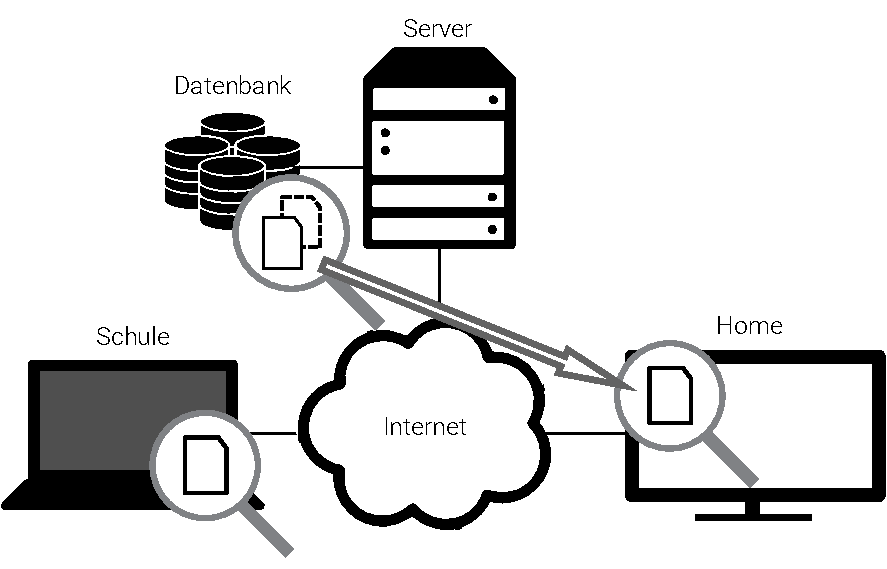
\includegraphics[]{images/dropbox_download}
  \caption{Üblich gehandhabtes Uploaden einer Datei}.
\end{figure}

Bei dem Erstellen und Bearbeiten des Übungsprotokolls auf dem Schulrechner in Form
einer Text-Datei wird eine Kopie Datei auf den vom Betreiber zur Verfügung gestellten
\gls{cloudstorage} beziehungsweise dessen Server hochgeladen und dort gespeichert.
Der Sender behält dabei die Originaldatei.

\begin{figure}[ht]
	\centering
  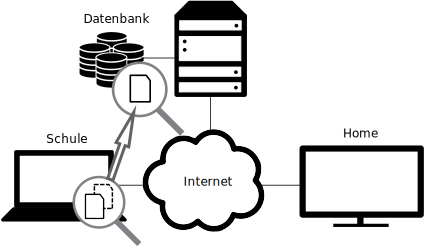
\includegraphics[]{images/dropbox_upload}
  \caption{Üblich gehandhabtes Downloaden einer Datei (wird noch geändert)}.
\end{figure}

Wenn der Heim-PC in diesem Beispiel hochgefahren ist, wird er
über die Änderung im \gls{cloudstorage} informiert und lädt die Änderung, in
diesem Fall die neuste Version des Übungsprotokoll von dem Server herunter.
Die Text-Datei wurde somit über die zentrale Stelle, hier den Server synchronisiert.

Das Übungsprotokoll hat nach dem Synchronistationsvorgang natürlich auf dem Heim-PC
den gleichen Inhalt wie die Datei auf dem Schulrechner, da es sich um die selbe Version
handelt. Wenn man das Übungsprotokoll nun dem Heim-PC bearbeiten würde, würde
die neue Version genauso wie vorhin zuerst auf den Server geladen werden und vom Server
aus auf die einzelnen Clients, hier nur auf den Schulrechner synchronisiert
werden und die neue Version des Übungsprotokoll überschreibt die alte.
